\subsection{Model Adaptation}\label{subsec:model-adaptation}
Our approach adapts DCRNN model~\cite{DCRNN} to take in consideration the wheelchair traffic.
This model captures the spatial dependency of traffic data using a custom diffusion convolution operation.
The temporal dependency is captured using Gated Recurrent Units (GRU) where matrix multiplications are replaced by
the diffusion convolution operation to create a Diffusion Convolution Gated Recurrent Unit (DCGRU).
We kept the encoder-decoder architecture of the DCRNN, but we modified some of the layers.
The model's architecture is shown in Fig.~\ref{fig:model}.
Such modifications are:

\begin{itemize}
    \item \textbf{DCGRU Cell}:
    The diffusion convolution operation in the DCGRU cell is replaced by a custom convolution that inherits from the
    MessagePassing class of the PyTorch Geometric library.
    \item \textbf{Attention Mechanism}:
    An attention mechanism is added to the model to allow the capture of different locomotion modes tendencies.
\end{itemize}
\vspace{1em}

The MessagePassing class is the base of building graph neural networks layers in PyTorch Geometric.
It allows our model to capture the spatial dependency of the graph traffic data.
It works by applying a function on features of neighboring nodes and aggregating the results, we use the addition as the
aggregation function.
It then combines the node features with the aggregated results using a fully connected layer to update the node
representation.
Attention mechanisms add trainable parameters that act like importance weights to the model.
Our model uses a multi-headed attention mechanism that allows it to differentiate between cars and wheelchairs.
\vspace{1em}

\begin{figure*}[htbp]
    \centering
    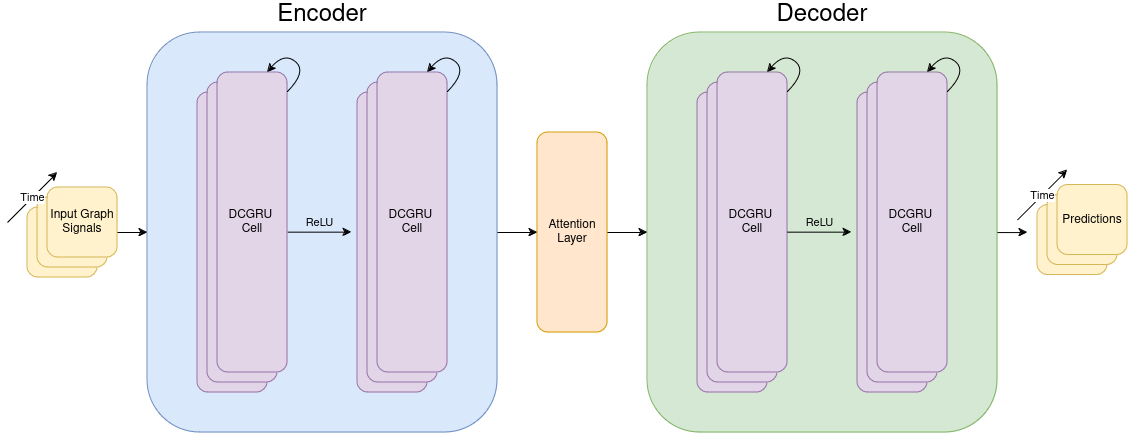
\includegraphics[width=1\textwidth]{images/model}
    \caption{
        Adapted DCRNN Model Architecture.
    }
    \label{fig:model}
\end{figure*}

\subsection{Derivation}\label{subsec:derivation}
Due to a massive lack of wheelchair traffic in the literature, this paper proposes a method to derive wheelchair data
from car traffic data.
METRopolitan Los Angeles (METR-LA) contains data about traffic information collected from loop detectors in the highway
of Los Angeles.
This dataset contains data about vehicle speed in miles per hour from 207 sensors, collected between March 1st, 2012 and
June 30th, 2012 that is aggregated into 5 minutes windows and normalized using Z-Score normalization.
From the data a graph is build using a weighted adjacency matrix $W$
where the weights represent the distance between the sensors, this matrix is build using a thresholded Gaussian kernel
weighting function~\cite{Shuman_2013}~\eqref{eq:tresholded_gaussian_kernel}.
Where $\text{dist}(i,j)$ is the distance between sensor $i$ and sensor $j$, $\sigma$
is the standard deviation of the distances and $\kappa$ is an arbitrary threshold.
\vspace{1em}

\begin{equation}
    W_{i,j} =
    \begin{cases}
        \exp\left( -\frac{\left[\text{dist}(i,j)\right]^2}{2\sigma^2} \right) & \text{if } \text{dist}(i,j) \leq \kappa
        \\
        0 & \text{otherwise}
    \end{cases}\label{eq:tresholded_gaussian_kernel}
\end{equation}
\vspace{1em}

We get accessibility data for each sensor we have using OpenStreetMap~\cite{OpenStreetMap}.
Every location in the database, either node, way or relation, can have tags that describe the location.
The tag we are interested in is the \textit{wheelchair} tag, it has 3 possible values: \textit{yes, limited, no}.
We look in a 500 meters radius around each sensor every accessibility tag and use~\eqref{eq:accessibility_score}
to compute an accessibility score for each sensor.
Where $x$ is the number of \textit{yes} tags and $y$ the number of \textit{no} tags in the circle area.
The sensor locations and search areas are shown in Fig.~\ref{fig:map}.
Equation~\eqref{eq:accessibility_score}, shown in Fig.~\ref{fig:accessibility_score_function}
,  allows areas that have more \textit{yes}
tags to have a higher score, while also rewarding areas that have more data available.

\begin{equation}
    f(x, y) = \frac{x}{x + y} \times \log(x + y + 1)\label{eq:accessibility_score}
\end{equation}
\vspace{1em}

\begin{figure}[htbp]
    \centering
    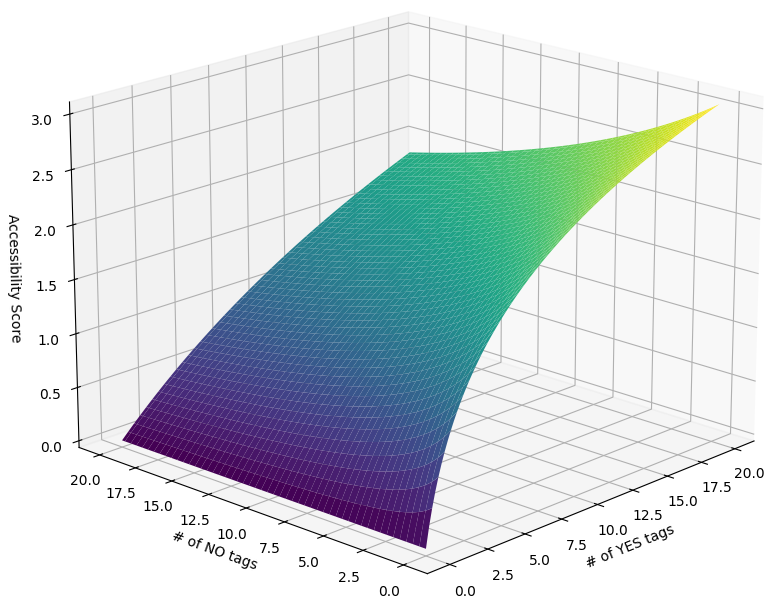
\includegraphics[width=0.5\textwidth]{images/accessibility_score_function}
    \caption{Accessibility score distribution of~\eqref{eq:accessibility_score}.}
    \label{fig:accessibility_score_function}
\end{figure}

\begin{figure}[htbp]
    \centering
    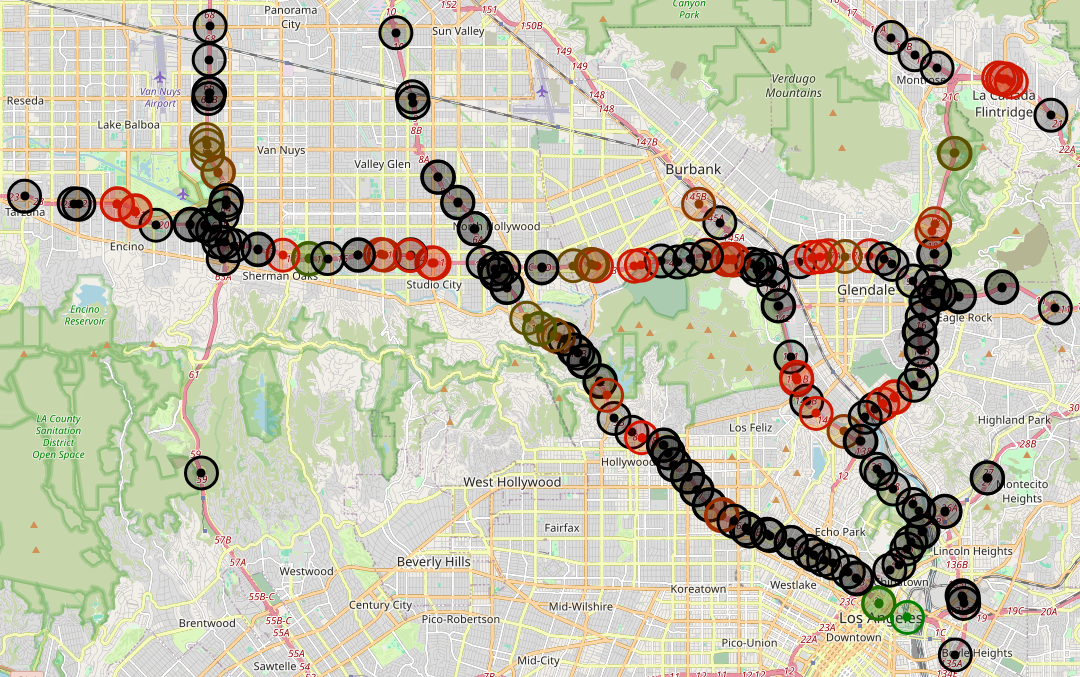
\includegraphics[width=0.5\textwidth]{images/map}
    \caption{
        Map of the sensors with their accessibility score and 500 meters radius around them.
        The sensors are colored based on their score, red being the lowest and green the highest.
        Every black sensor indicates that there is no accessibility data available.
    }
    \label{fig:map}
\end{figure}

We apply a linear transformation to the original traffic speed data to get wheelchair speeds between 0 and 4, where 4 is
a value from~\cite{FreedomMobility}.
We add some noise to the data to slightly change the values and make the model more robust.
We finally multiply our values by the accessibility score and apply a min/max scaling to end with values between 0 and
4.

\subsection{Training}\label{subsec:training}
The implementation uses PyTorch, PyTorch Geometric, PyTorch Lightning and WandB for monitoring.
We split the data into a training (70\%), validation (10\%) and test (20\%) sets.
The inputs are shaped as follows: (number of samples, number of sensors, sequence length, number of features) e.g. (
29977, 207, 12, 4).
We do not normalize the speed feature.
The sequence length is 12, which corresponds to 1 hour of data and the features are:

\begin{itemize}
    \item speed (in miles per hour)
    \item hour of the day
    \item day of the week
    \item locomotion mode (hot encoded)
\end{itemize}
\vspace{1em}

The model is evaluated using three metrics:
\begin{itemize}
    \item Mean Absolute Error (MAE)~\eqref{eq:mae}
    \item Root Mean Squared Error (RMSE)~\eqref{eq:rmse}
\end{itemize}
Where $y$ is the ground truth, $\hat{y}$ the prediction and $n$ the batch size.

\begin{equation}
    MAE(y, \hat{y}) = \frac{1}{n} \sum_{i=1}^{n} \left| y_i - \hat{y}_i \right|\label{eq:mae}
\end{equation}

\begin{equation}
    RMSE(y, \hat{y}) = \sqrt{\frac{1}{n} \sum_{i=1}^{n} \left( y_i - \hat{y}_i \right)^2}\label{eq:rmse}
\end{equation}
\vspace{1em}